\documentclass[conf]{new-aiaa}
%\documentclass[journal]{new-aiaa} for journal papers
\usepackage[utf8]{inputenc}

\usepackage{graphicx}
\usepackage{amsmath}
\usepackage[version=4]{mhchem}
\usepackage{siunitx}
\usepackage{longtable,tabularx}
\usepackage{footnote}
\usepackage{mhchem}
\usepackage{physics}
\usepackage{array,makecell,booktabs}
\newcolumntype{M}[1]{>{\centering\arraybackslash}m{#1}}
\usepackage[super]{nth}
\makesavenoteenv{tabular}
\setlength\LTleft{0pt}

\graphicspath{{figures/}}

\begin{document}

\section{Performance Model}

Overall payload mass fraction is the key performance metric for launch vehicles. It determines how large a vehicle is needed to launch a given payload. As larger launch vehicle are generally more expensive, higher payload mass fractions are preferable. This section describes a quick method for estimating the payload capacity of 2-stage launch vehicles with reusable first stages, suitable for preliminary design work.

The payload mass fraction $\pi_*$ is defined as:

\begin{equation}
\pi_* \equiv \frac{m_*}{m_0}
\end{equation}

where $m_*$ is the (maximum) payload mass and $m_0$ is the gross (wet) liftoff mass of the vehicle, including payload, all stages and propellant.

Payload performance depends on the target orbit and on the design of the launch vehicle. The relation between vehicle design, payload capacity, and the $\Delta v$ required to reach the target orbit can be derived from Newtonian mechanics and is expressed by Tsiolkovsky’s rocket equation. The $\Delta v$ capability of a single stage is\footnote{The form of Tsiolkovsky's equation used here is taken from \cite{Wiesel2010}}:

\begin{equation}
\Delta v_i = - I_{sp,i} g_0 \ln \left( \epsilon_i + (1 - \epsilon_i) \pi_i \right)
\end{equation}

where $I_{sp,i}$ is the (average) specific impulse of the $i$-th stage engines, $\epsilon_i$ is the inert mass fraction of the $i$-th stage, and $\pi_i$ is the payload mass fraction of the $i$-th stage. The inert mass fraction is the stage's inert mass divided by its wet mass:

\begin{equation}
\epsilon_i \equiv \frac{m_{inert,i}}{m_i} = \frac{m_{inert,i}}{m_{inert,i} + m_{p,i}}
\end{equation}

The payload mass fraction of a \emph{stage} is:
\begin{equation}
\pi_i \equiv \frac{\sum_{j=i+1}^N (m_j) + m_*}{m_i + \sum_{j=i+1}^N (m_j) + m_*}
\end{equation}

where $\sum_{j=i+1}^N (m_j) + m_*$ is the mass of the upper stages and payload carried by stage $i$.

For a two stage launch vehicle, we introduce an additional parameter, $y$, the stage 1 / stage 2 wet mass ratio:

\begin{equation}
y \equiv \frac{m_2}{m_1}
\end{equation}

For current U.S. 2-stage launch vehicles, values of $y$ are 0.076 to 0.265. Lower values of $y$ result in a higher staging velocity for a given mission and there is a value of $y$ which maximizes $\pi_*$ if the other parameters are fixed.

Then, Tsiolkovsky’s relation can be written as the following system of equations:

\begin{equation}
% TODO multiline equation align equals signs
\label{eq:dv_2_stage}
\Delta v_* = \Delta v_1 + \Delta v_2
           = - I_{sp,1} g_0 \ln \left( \epsilon_1 + (1 - \epsilon_1) \pi_1 \right)
             - I_{sp,2} g_0 \ln \left( \epsilon_2 + (1 - \epsilon_2) \pi_2 \right)
\end{equation}

\begin{equation}
\label{eq:ypi}
\pi_2 = (y + 1) - \frac{y}{\pi_1}
\end{equation}

\begin{equation}
\label{eq:pi_prod}
\pi_* = pi_1 pi_2
\end{equation}

A given launch vehicle design is represented by the parameters $(I_{sp,1}, I_{sp,2}, \epsilon_1, \epsilon_2, y)$. Given these parameters and a target orbit, we find the payload performance of the launch vehicle by:

\begin{enumerate}
    \item fixing $\Delta v_*$ to the $\Delta v_*$ required to reach the target orbit from the launch site, including losses.
    \item solving (numerically) the system of equations (\ref{eq:dv_2_stage}-\ref{eq:pi_prod}) for $pi_*$
\end{enumerate}

To validated the model, calculations were run for the Delta IV M and Falcon 9 Block 3 (expendable configuration) launch vehicles [Figure \ref{fig:payload_vs_dv}]. The advertised payload mass fractions for LEO and GTO are shown (crosses) for comparison. The model slightly over-predicts $\pi_*$, likely because it neglects the mass of the payload fairing.

\begin{figure}[hbt!]
    \centering
    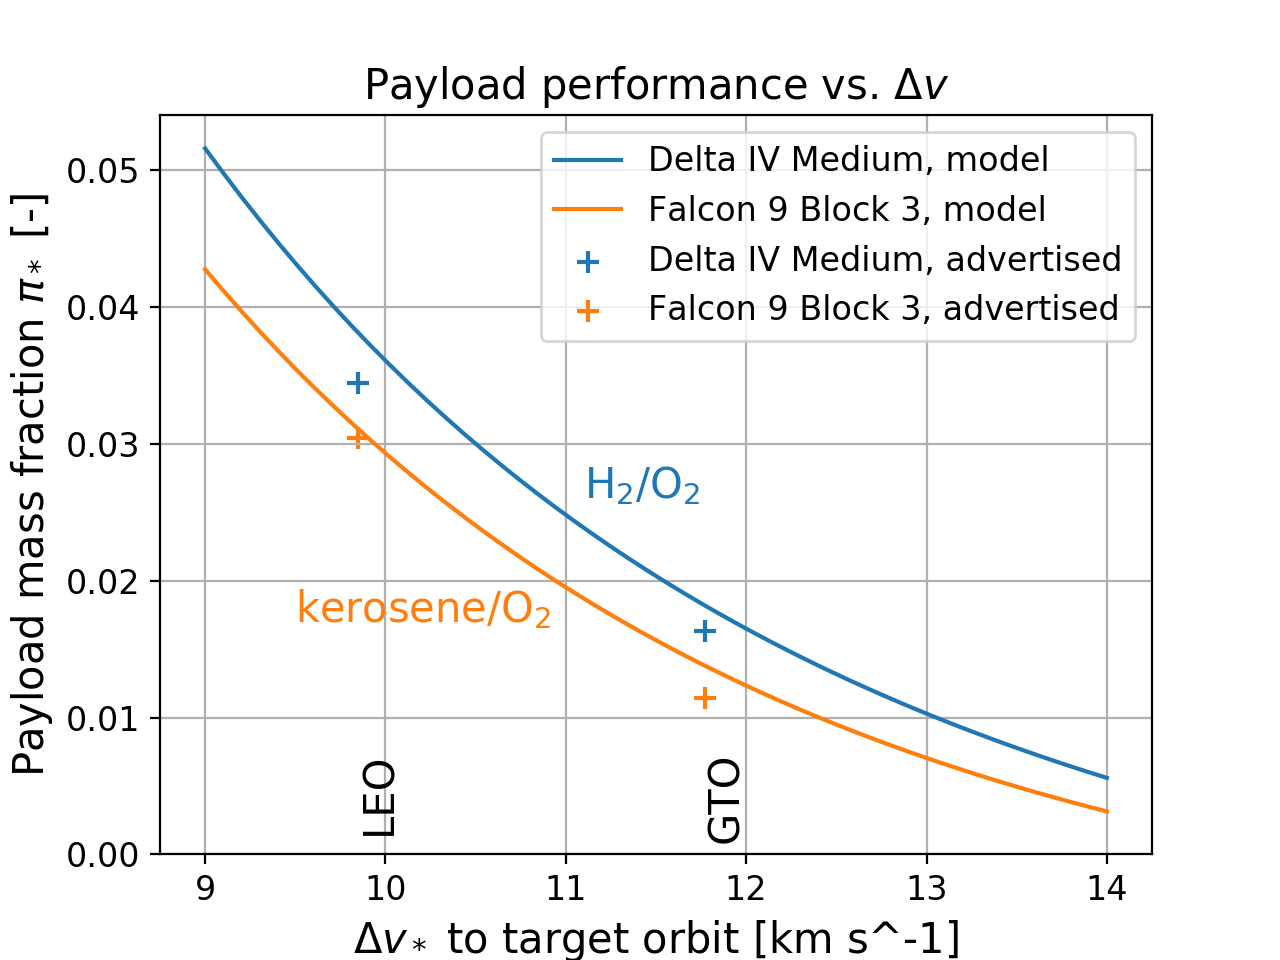
\includegraphics[width=\textwidth]{../../lvreuse/analysis/performance/plots/payload_vs_dv}
    \caption{\label{fig:payload_vs_dv} The quick model makes reasonably accurate predictions of the payload capacity of two expendable launch vehicles. Payload performance declines with increasing $\Delta v_*$, and is slightly higher for \ce{H_2} fueled vehicles than for kerosene vehicles.}
\end{figure}

\subsection{Technology choice}
Clearly, payload performance depends on inert mass fraction and specific impulse, and would be maximized for $\epsilon \rightarrow 0, \quad I_{sp} \rightarrow \infty$. However, there are technological limits on the achievable values, which depend on a collection of design decisions, i.e. the propellant, engine cycle, tank and structure materials, etc. We refer to this collection of decisions as a "technology choice". The technology choice sets $I_{sp, 1}, I_{sp, 2}$, and sets lowers feasible limits for the inert mass fractions, which we will call $E_1, E_2$. The technology choice also influences the cost model (see next section). We will analyze reuse strategies under two example technology choices:

\begin{itemize}
    \item \ce{H2} / \ce{O2} propellants, staged combustion cycle, aluminum alloy tanks
    \item kerosene / \ce{O2} propellants, gas generator cycle, aluminum alloy tanks
\end{itemize}

These technologies are mature and have had fairly consistent specific impulse and inert mass limits over the past 30 years\footnote{This analysis can easily be extended to new technologies, e.g. \ce{CH4} / \ce{O2} propellants or composite tanks, as the engineering limits on these technologies emerge}. Stages using hydrogen technology have higher $I_{sp}$ but higher feasible inert mass $E$ than those using kerosene. The balance of these effects works out to slightly favor hydrogen in terms of payload performance [Figure \ref{fig:payload_vs_dv}]. Finally, note that the technology choice and reuse strategy are independent - any reuse strategy can conceivably be used with any technology choice.


\subsection{How first stage reuse effects performance}
So far we have reviewed the factors determining launch vehicle performance. Now we ask, how does first stage reuse change these factors? Two mechanisms are possible:

\begin{itemize}
    \item \emph{$\Delta v$ losses} - Some reuse strategies require modifying the outer mold line of the stage or altering the ascent trajectory. This changes the drag, gravity and steering losses during ascent, and could cause the $\Delta v_*$ to a target orbit to be different for reusable and expendable strategies.
    \item \emph{Extra mass on the first stage} - All reuse strategies require the first stage to carry some extra mass during ascent, as extra hardware (landing gear, wings, etc.) and/or as propellant reserved for recovery.
\end{itemize}

Fortunately, the first can be ignored, as the variation of losses for different recovery strategies is minor and comparable to the variation in losses for fully expendable vehicles \cite{Stappert2017}. Thus, the main effect of first stage reuse on performance is that extra mass must be carried during ascent.

\subsection{First stage unavailable mass}
We define the "first stage unavailable mass fraction", $\epsilon_1'$, to be the fraction of first stage gross mass that is unavailable to be expelled during ascent, i.e.:

\begin{equation}
\label{eq:epsilon_1_prime}
\epsilon_1' = \frac{m_{inert,1} + m_{pr,1}}{m_{inert,1} + m_{p,1}}
\end{equation}

where $m_{pr,1}$ is the mass of propellant reserved for recovery maneuvers, and $m_{p,1}$ is the total stage 1 propellant mass.
The payload performance of a vehicle with first stage reuse can be found by substituting $\epsilon_1'$ for $\epsilon_1$ in Equation \ref{eq:dv_2_stage}, and solving Equations \ref{eq:dv_2_stage}-\ref{eq:pi_prod}. 

\subsection{Relating unavailable mass to recovery hardware and propulsion}
Next, we relate $\epsilon_1'$ to the feasible limit on inert mass ($E_1$) and the extra hardware and propellant needed for recovery.
It will be helpful to compare the mass of the first stage to a "baseline" mass, $m_{hb,1} = TODO$

Then, we define three new dimensionless variables:
\begin{itemize}
    \item $z_m$ is the fraction of the first stage baseline mass which is recovered
\end{itemize}
define

\subsection{Estimating hardware and propulsion for recovery strategies}
introduce/review Monte Carlo method
refer to appendix for derivation of input distributions
show e vs P, a contour plot

\subsection{Payload fraction estimates for recovery strategies}
show violin plots

\bibliography{first_stage_recovery}

\end{document}